\documentclass[a4paper]{scrartcl}
\usepackage[cm]{fullpage}
\usepackage{amsmath, amssymb, esint}
\usepackage{siunitx}

\usepackage{tikz, pgfplots}
\pgfplotsset{
    compat = 1.12,
    plot-scatter/.style = {
        only marks,
        mark size = 0.8
    }
}

\begin{document}

\title{PHYS2114: RLC Circuits}
\author{ \\ \\ }
\date{2016-09-20}
\maketitle

\section{Introduction}
Please refer to the student notes of the experiment.

\section{Materials and Methods}
Please refer to the student notes, operating instructions and prework of the experiment.

A TBS 1072B-EDU (\SI{1}{\mega\ohm} in parallel with \SI{20}{\pico\farad} input) oscilloscope was used to collect numerical data, while a Farnell LFP1 PSU using its Low-Z (\SI{3}{\ohm}) output was our signal generator.

All cable runs between components were twisted pairs to reduce stray inductance, since no short length cable was available.

The capacitor in the circuit was labelled \SI{0.047}{\micro\farad}, and assumed to be accurate.

Data was fitted to the expected curves using the Mathematica 10.2 function \texttt{FindFit[]} without any options.

\subsection{Part 1}
Three different resistances were used, where the resistance across the capacitor (with the PSU shorted) was \SI{6.8}{\ohm}, \SI{11.6}{\ohm} and \SI{17.0}{\ohm}. The square wave output of the PSU was set to \SI{160.00 \pm 0.05}{\hertz}. Each resistance had the measurements taken with RMS voltages of \SI{1}{\volt}, \SI{2}{\volt} and \SI{4}{\volt}.

The time-voltage points was fitted to the following function:
\[A e^{-k t} \sin(\omega t + \phi) + b\]
where the oscillation frequency is \(f_1 = \frac{\omega}{2 \pi}\).

\subsection{Part 2}
The resistor was measured to have resistance \SI{5.0}{\ohm}, while with the resistor and PSU shorted, resistance across the capacitor was \SI{6.7}{\ohm}. For simplicity, this extra resistance as modelled purely as resistance in the inductor (i.e., the connecting cables were assumes to be perfect conductors).

The time-voltage points was fitted to the following function:
\[A \sin(\omega t + \phi) + b\]
and then aggregated together to form an empirical transfer function.

\section{Results}
\subsection{Part 1}
\begin{table}
    \centering
    \begin{tabular}{c | c | c}
        \(R\) (\si{\ohm}) & \(k\) (\si{\per\second}) & \(f_1\) (\si{\hertz}) \\
        \hline
        6.8 & \SI{22220 \pm 90}{} & \SI{79340 \pm 30}{} \\
        11.6 & \SI{22360 \pm 30}{} & \SI{79334 \pm 12}{} \\
        17.0 & \SI{22400 \pm 200}{} & \SI{79355 \pm 4}{} \\
        (All) & \SI{22300 \pm 200}{} & \SI{79340 \pm 30}{}
    \end{tabular}
    \caption{Damping constants and oscillation frequencies}
    \label{tab:part1}
\end{table}
\begin{figure}
    \centering
    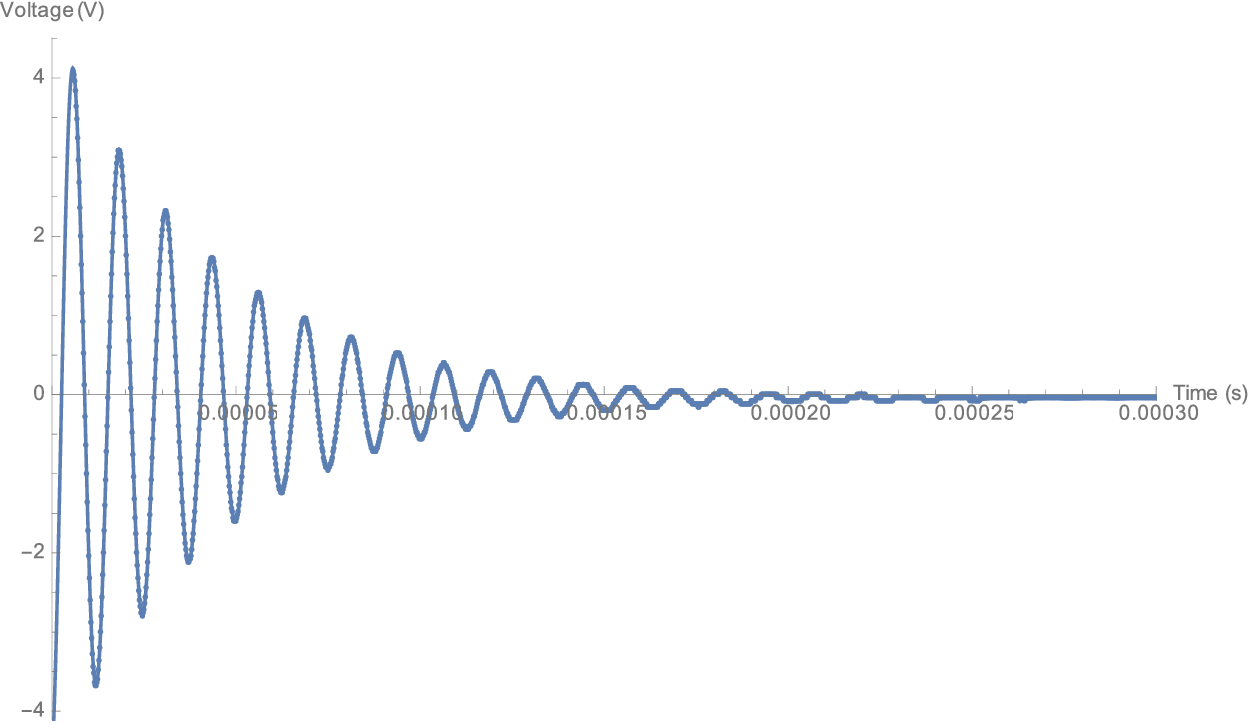
\includegraphics[width = 18cm]{part1-example.png}
    \caption{Example of the recorded data and fitted curve}
    \label{fig:part1-example}
\end{figure}

The damping constant and oscillation frequencies extracted from the data is shown in Table \ref{tab:part1}. An example of the data and fit is shown in Figure \ref{fig:part1-example}.

Assuming an inductance of \SI{2.56}{\milli\henry} (from the student notes, since the inductor wasn't labelled), the theoretical damping constants are \SI{2660}{\per\second}, \SI{4530}{\per\second} and \SI{6640}{\per\second} for resistances of \SI{6.8}{\ohm}, \SI{11.6}{\ohm} and \SI{17.0}{\ohm}, respectively. Meanwhile, the oscillation frequency is \SI{14.5}{\kilo\hertz}.

\subsection{Part 2}
\begin{figure}
    \centering
    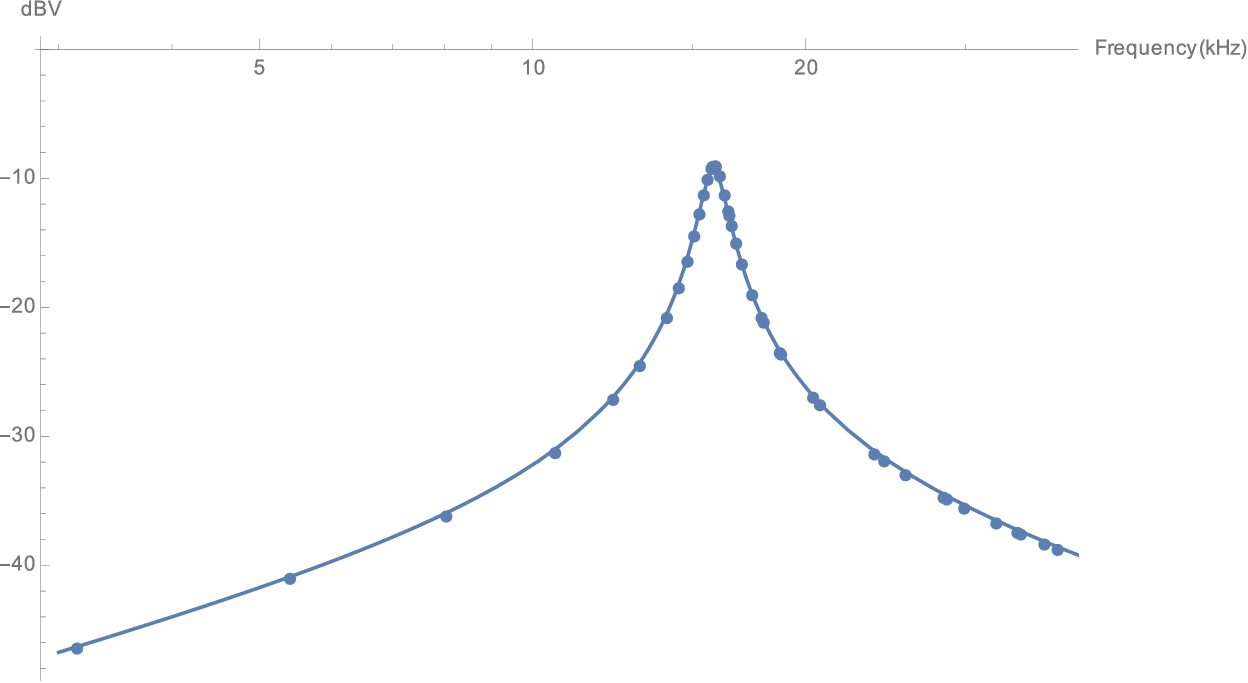
\includegraphics[width = 18cm]{part2-mag.png}
    \caption{Transfer function magnitude with fitted curve}
    \label{fig:part2-mag}
\end{figure}
\begin{figure}
    \centering
    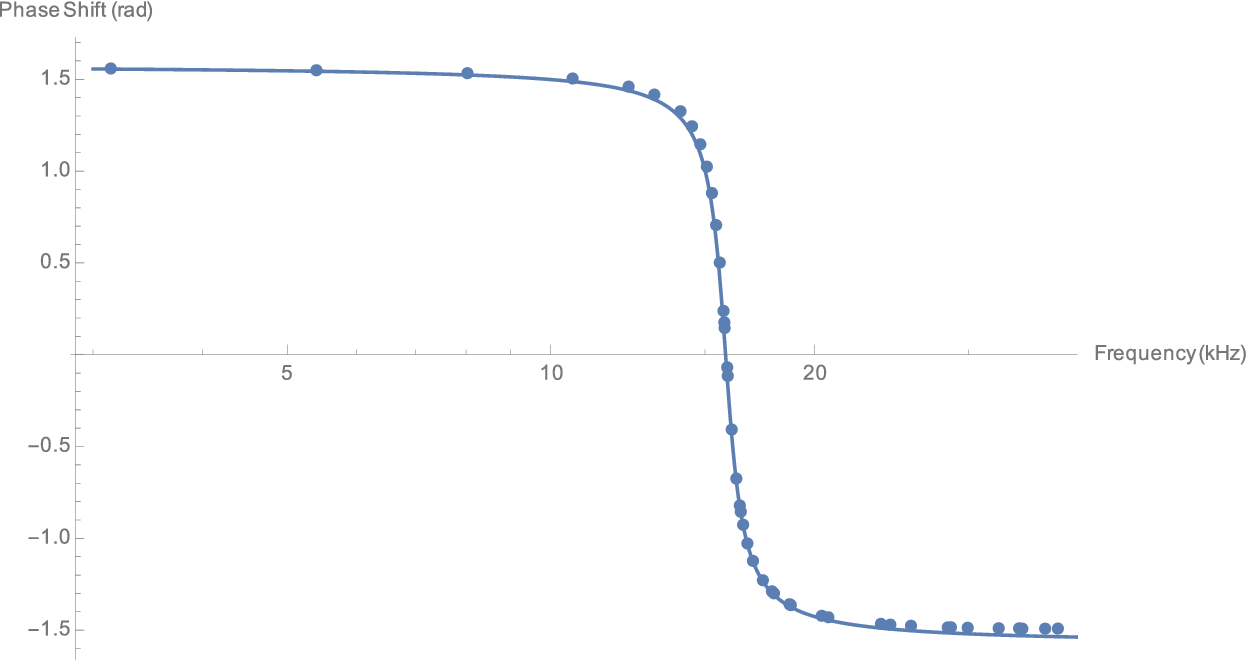
\includegraphics[width = 18cm]{part2-arg.png}
    \caption{Transfer function argument with fitted curve}
    \label{fig:part2-arg}
\end{figure}

The measured transfer function is shown in Figures \ref{fig:part2-mag} and \ref{fig:part2-arg}. The theoretical transfer function with an inductance of \SI{2.15 \pm 0.03}{\milli\henry} is plotted alongside it.

The resonant frequency is \(f_0 = \SI{15.8 \pm 0.1}{\kilo\hertz}\) with a bandwidth of \(\Delta f = \SI{1.1 \pm 0.1}{\kilo\hertz}\), corresponding to a Q-factor of \(Q = \SI{14 \pm 1}{}\). Meanwhile, the theoretical values are \(f_0 \approx \SI{15.83}{\kilo\hertz}\), \(\Delta f \approx \SI{1.09}{\kilo\hertz}\) and \(Q \approx \SI{14.5}{}\).

\section{Discussion}
\subsection{Part 1}
Immediately one can see in Table \ref{tab:part1} that it doesn't match the expected behaviour of the circuit. The damping constant \(k\) did not increase proportionally with resistance. The values themselves were of the wrong order of magnitude from the theoretical values as well, despite the expected curve fitting the recorded data excellently, as can be seen in Figure \ref{fig:part1-example}.

Most likely, there was an issue with the experimental setup. While I have no explanation for why the damping constant doesn't change across resistances, the high oscillation frequency would be the inductor or capacitor having a much higher value than expected, or some significant stray inductance/capacitance in the circuit.

\subsection{Part 2}
From both the transfer functions themselves in Figures \ref{fig:part2-mag} and \ref{fig:part2-arg}, as well as the standard filter metrics as stated above, the experimental values come to a good agreement with the theoretical ones.

While there appears to be a small systematic shift in values in frequencies away from the resonant frequency, this shift is small, and is likely attributable to the non-idealness of the components used.

\section{Conclusion}
\subsection{Part 1}
The measured damping constant and oscillation frequencies of the freely-oscillating RLC circuit is shown in Table \ref{tab:part1}, with an example of the waveform in Figure \ref{fig:part1-example}. However, the theoretical values are an order of magnitude smaller, so this result is probably rubbish.

\subsection{Part 2}
The measured resonant frequency of the RLC circuit is \(f_0 = \SI{15.8 \pm 0.1}{\kilo\hertz}\) with a bandwidth of \(\Delta f = \SI{1.1 \pm 0.1}{\kilo\hertz}\), corresponding to a Q-factor of \(Q = \SI{14 \pm 1}{}\). This is in good agreement with the theoretical values of \(f_0 \approx \SI{15.83}{\kilo\hertz}\), \(\Delta f \approx \SI{1.09}{\kilo\hertz}\) and \(Q \approx \SI{14.5}{}\), where an inductor of inductance \SI{2.15 \pm 0.03}{\milli\henry} is used. This agreement can further be seen in the transfer function plots in Figures \ref{fig:part2-mag} and \ref{fig:part2-arg}.

\end{document}